% !TEX program = xelatex
% Compile with XeLaTeX (latexmk reads .latexmkrc in this folder): the Ubuntu fonts need fontspec
\documentclass[aspectratio=169,10pt]{beamer}
\usetheme{metropolis}
\usepackage{amsmath}
% Ubuntu everywhere: text, monospace (Ubuntu Mono) and, in the formulas, letters, digits, Greek and the
% common operators (= + - x <= ...). Only the symbols that Ubuntu does not have (big sum, arrows,
% calligraphic letters) come from the sans-serif math font TeX Gyre DejaVu Math.
% fonts/ holds static instances of the Ubuntu fonts (Ubuntu Font Licence, fonts/LICENCE.txt): the system
% files are variable fonts, of which XeLaTeX embeds only the regular weight.
\usefonttheme{professionalfonts}
\usepackage{fontspec}
\usepackage{unicode-math}
\defaultfontfeatures{Path=fonts/, Extension=.ttf}
\setsansfont{Ubuntu}[UprightFont=*-Regular, BoldFont=*-Bold, ItalicFont=*-Italic, BoldItalicFont=*-BoldItalic]
\setmainfont{Ubuntu}[UprightFont=*-Regular, BoldFont=*-Bold, ItalicFont=*-Italic, BoldItalicFont=*-BoldItalic]
\setmonofont{UbuntuMono}[UprightFont=*-Regular, BoldFont=*-Bold, ItalicFont=*-Italic, BoldItalicFont=*-BoldItalic]
\setmathfont{texgyredejavu-math.otf}[Path=, Extension=]
\setmathfont{Ubuntu-Regular}[range={up/{Latin,latin,num,Greek,greek},"2B,"3D,"28,"29,"5B,"5D,"2F,"7C,"2212,"D7,"2264,"2265,"2248,"221E,"3C,"3E,"2C,"3A,"3B,"21,"2026,"2032}]
\setmathfont{Ubuntu-Italic}[range={it/{Latin,latin}}]
\setmathfont{Ubuntu-Regular}[range={it/{Greek,greek}}] % upright Greek: the italic pi of Ubuntu looks like an n
\setmathfont{Ubuntu-Bold}[range={bfup/{Latin,latin,num,Greek,greek}}]
\setmathrm{Ubuntu}[UprightFont=*-Regular, BoldFont=*-Bold, ItalicFont=*-Italic, BoldItalicFont=*-BoldItalic]
\setoperatorfont\mathrm
\renewcommand{\familydefault}{\sfdefault}
\setbeamerfont{title}{family=\sffamily}
\usepackage{booktabs}
\usepackage{tikz}
\usetikzlibrary{positioning,arrows.meta,calc}
\usepackage{xcolor}

\definecolor{accent}{HTML}{E65100}   % deep orange
\definecolor{accentdark}{HTML}{BF360C}
\definecolor{good}{HTML}{2E7D32}
\definecolor{bad}{HTML}{B71C1C}
\setbeamercolor{palette primary}{bg=accent,fg=white}       % frame titles, standout slide
\setbeamercolor{frametitle}{bg=accent,fg=white}
\setbeamercolor{progress bar}{fg=accent,bg=accent!20}
\setbeamercolor{title separator}{fg=accent}
\setbeamercolor{structure}{fg=accentdark}                  % bullets, description labels
\setbeamercolor{section in toc}{fg=accentdark}
\setbeamercolor{alerted text}{fg=bad}
\setbeamercolor{background canvas}{bg=white}

\newcommand{\vseq}{\texttt{baseline-sequential}}
\newcommand{\vbase}{\texttt{baseline-MPI-OpenMP}}
\newcommand{\optone}{\texttt{opt1}}
\newcommand{\opttwo}{\texttt{opt2}}
\newcommand{\plot}[2][0.86]{\centering\includegraphics[width=#1\textwidth]{../../results/plots/#2}}
\newcommand{\perfplot}[1]{\begin{center}\includegraphics[width=0.65\textwidth]{../../results/plots/performance/#1.pdf}\end{center}\vspace{-1.4em}\small}
\newcommand{\takeaway}[1]{\begin{center}\colorbox{accent!10}{\parbox{0.92\textwidth}{\centering\small #1}}\end{center}}

\title{Parallel Expectation--Maximization Clustering}
\subtitle{Hybrid MPI + OpenMP EM for Gaussian mixtures, diagonal and full covariance}
\author{%
\textbf{Group 6}\\[4pt]
\begin{tabular}[t]{@{}l@{}}
Michael Bernasconi\\
{\scriptsize Student ID: 267681}\\
{\scriptsize\texttt{michael.bernasconi@studenti.unitn.it}}
\end{tabular}\hspace{3em}%
\begin{tabular}[t]{@{}l@{}}
Gabriele Fronzoni\\
{\scriptsize Student ID: 267336}\\
{\scriptsize\texttt{gabriele.fronzoni@studenti.unitn.it}}
\end{tabular}}
\institute{High Performance Computing --- Department of Information Engineering and Computer Science, University of Trento\\[2pt]
\scriptsize\url{https://github.com/HPC-2627/ParallelExpectationMaximizationClustering}}
\date{}


% Section divider slides: orange panel with the section number, Gaussian contours, title and progress bar
\newif\ifbackup
\newcommand{\nmainsections}{5}
\setbeamertemplate{section page}{%
\begin{tikzpicture}[remember picture,overlay]
\begin{scope}[shift={(current page.south west)}]
  \fill[accent] (0,0) -- (5.7,0) -- (4.5,9) -- (0,9) -- cycle;
  \fill[accent!35] (5.95,0) -- (6.45,0) -- (5.25,9) -- (4.75,9) -- cycle;
  \fill[accentdark] (0,0) -- (3.0,0) -- (0,2.7) -- cycle;
  \fill[accentdark!80!black,opacity=0.35] (0,9) -- (2.2,9) -- (0,7.4) -- cycle;
  \begin{scope}
    \clip (0,0) -- (5.7,0) -- (4.5,9) -- (0,9) -- cycle;
    \pgfmathsetseed{7}
    \foreach \cx/\cy/\r/\a/\b in {3.3/7.4/28/0.75/0.38, 1.2/5.9/-30/0.55/0.32, 3.7/1.7/55/0.7/0.35} {
      \draw[white,opacity=0.45,line width=0.8pt,rotate around={\r:(\cx,\cy)}] (\cx,\cy) ellipse [x radius={2*\a}, y radius={2*\b}];
      \draw[white,opacity=0.3,line width=0.5pt,dashed,rotate around={\r:(\cx,\cy)}] (\cx,\cy) ellipse [x radius=\a, y radius=\b];
      \foreach \i in {1,...,22} {
        \pgfmathsetmacro{\u}{0.75*\a*(rand+rand)}
        \pgfmathsetmacro{\v}{0.75*\b*(rand+rand)}
        \fill[white,opacity=0.55] ({\cx+\u*cos(\r)-\v*sin(\r)},{\cy+\u*sin(\r)+\v*cos(\r)}) circle (0.9pt);
      }
    }
  \end{scope}
  % big section number
  \node[white,font=\fontsize{64}{64}\selectfont\bfseries] at (2.55,4.5) {\ifbackup B\else 0\arabic{section}\fi};
  % title on the right
  \node[anchor=south west,text width=8.4cm,inner sep=0pt] at (7.1,4.75) {%
    {\color{accent}\footnotesize\bfseries \ifbackup APPENDIX\else SECTION 0\arabic{section}\fi\par}\vspace{4pt}
    {\usebeamercolor[fg]{normal text}\fontsize{22}{26}\selectfont\bfseries\raggedright\hyphenpenalty=10000 \insertsectionhead\par}};
  \draw[accent,line width=1.2pt] (7.1,4.45) -- (11.1,4.45);
  % progress bar: one block per main section
  \ifbackup
    \node[anchor=north west,inner sep=0pt,font=\scriptsize,text=accentdark] at (7.1,4.1) {Extra material for the questions};
  \else
    \foreach \k in {1,...,\nmainsections} {
      \ifnum\k=\value{section}\def\blk{accent}\else\ifnum\k<\value{section}\def\blk{accent!55}\else\def\blk{accent!15}\fi\fi
      \fill[\blk] ({7.1+0.62*(\k-1)},3.95) rectangle ++(0.5,0.13);
    }
  \fi
  % small triangles bottom right
  \foreach \k in {0,...,5} \fill[accent,opacity={1-0.15*\k}] ({14.9-0.3*\k},0.35) -- ({15.1-0.3*\k},0.35) -- ({15.0-0.3*\k},0.53) -- cycle;
\end{scope}
\end{tikzpicture}}

\begin{document}

% Title slide: custom layout, right panel drawn as a Gaussian mixture (ellipses = 1 and 2 sigma contours, dots = points)
\begin{frame}[plain]
\begin{tikzpicture}[remember picture,overlay]
\begin{scope}[shift={(current page.south west)}]
  % --- right panel: slanted orange shapes
  \fill[accent!35] (9.55,9) -- (10.15,9) -- (11.55,0) -- (10.95,0) -- cycle;
  \fill[accent] (10.4,9) -- (16,9) -- (16,0) -- (11.8,0) -- cycle;
  \fill[accentdark] (13.4,0) -- (16,0) -- (16,3.6) -- cycle;
  \fill[accentdark!80!black,opacity=0.35] (16,9) -- (16,6.3) -- (13.9,9) -- cycle;
  \begin{scope}
    \clip (10.4,9) -- (16,9) -- (16,0) -- (11.8,0) -- cycle;
    \pgfmathsetseed{42}
    % cluster: centre x, centre y, rotation, sigma a, sigma b, dot colour
    \foreach \cx/\cy/\r/\a/\b/\col in {
        12.55/6.75/30/0.55/0.28/white,
        14.75/7.35/-25/0.42/0.30/accent!15,
        14.05/4.45/62/0.72/0.32/white,
        12.65/2.55/-35/0.50/0.30/accent!15,
        15.05/1.55/12/0.38/0.26/white} {
      \draw[white,line width=0.9pt,rotate around={\r:(\cx,\cy)}] (\cx,\cy) ellipse [x radius={2*\a}, y radius={2*\b}];
      \draw[white,opacity=0.55,line width=0.6pt,dashed,rotate around={\r:(\cx,\cy)}] (\cx,\cy) ellipse [x radius=\a, y radius=\b];
      \foreach \i in {1,...,34} {
        \pgfmathsetmacro{\u}{0.75*\a*(rand+rand)}
        \pgfmathsetmacro{\v}{0.75*\b*(rand+rand)}
        \fill[\col,opacity=0.9] ({\cx+\u*cos(\r)-\v*sin(\r)},{\cy+\u*sin(\r)+\v*cos(\r)}) circle (0.95pt);
      }
      \draw[white,line width=1.4pt] (\cx-0.09,\cy-0.09) -- (\cx+0.09,\cy+0.09) (\cx-0.09,\cy+0.09) -- (\cx+0.09,\cy-0.09);
    }
    % background noise points
    \foreach \i in {1,...,40} {
      \fill[white,opacity=0.35] ({10.6+5.4*(rand+1)/2},{9*(rand+1)/2}) circle (0.7pt);
    }
  \end{scope}
  % --- left side: small geometric accents
  \fill[accent] (0.75,7.95) rectangle (0.86,6.35);
  \foreach \k in {0,...,5} \fill[accent,opacity={1-0.15*\k}] ({1.05+0.3*\k},0.35) -- ({1.25+0.3*\k},0.35) -- ({1.15+0.3*\k},0.53) -- cycle;
  % --- text
  \node[anchor=north west,text width=9.2cm,inner sep=0pt] at (1.05,7.95) {%
    {\usebeamercolor[fg]{title}\fontsize{14}{17}\selectfont\bfseries\mbox{Parallel Expectation--Maximization}\\ Clustering\par}
    \vspace{5pt}
    {\color{accentdark}\small Hybrid MPI + OpenMP EM for Gaussian mixtures,\\ diagonal and full covariance\par}
    \vspace{7pt}
    {\color{accent}\rule{5cm}{1.2pt}\par}
    \vspace{9pt}
    {\color{accent}\small\bfseries GROUP 6\par}\vspace{5pt}
    {\small\mbox{%
    \begin{tabular}[t]{@{}l@{}}
    \textbf{Michael Bernasconi}\\[0pt]
    {\scriptsize Student ID: 267681}\\[-1pt]
    {\scriptsize michael.bernasconi@studenti.unitn.it}
    \end{tabular}\hspace{1.4em}%
    \begin{tabular}[t]{@{}l@{}}
    \textbf{Gabriele Fronzoni}\\[0pt]
    {\scriptsize Student ID: 267336}\\[-1pt]
    {\scriptsize gabriele.fronzoni@studenti.unitn.it}
    \end{tabular}}\par}
    \vspace{12pt}
    {\scriptsize High Performance Computing\\
    Department of Information Engineering and Computer Science\\
    University of Trento\\[3pt]
    {\scriptsize\color{accentdark}\mbox{\url{https://github.com/HPC-2627/ParallelExpectationMaximizationClustering}}}\par}
  };
\end{scope}
\end{tikzpicture}
\end{frame}

\begin{frame}{Outline}
\tableofcontents
\end{frame}

% =====================================================================
\section{Problem}

\begin{frame}{Goal of the project}
\begin{itemize}
\item \textbf{Clustering} with a \textbf{Gaussian mixture model} (GMM): every point comes from one of $K$ Gaussians, the label is hidden.
\item Parameters estimated with the \textbf{Expectation--Maximization} (EM) algorithm: iterative, every iteration scans the \emph{whole} dataset $\Rightarrow$ cost grows with $N$.
\item \textbf{Goal}: implement EM in C with a \textbf{hybrid MPI + OpenMP} design, evaluate one optimization of the \emph{computation} and one of the \emph{communication}, measure \textbf{strong and weak scaling} on the HPC3 cluster (up to 4 nodes, 32 cores).
\item Two covariance models, \textbf{same importance}, never compared with each other:
  \begin{itemize}
  \item \textbf{diagonal}: one variance per variable, $O(NKD)$ per iteration (memory-bound);
  \item \textbf{full}: complete $D\times D$ matrix (Cholesky), $O(NKD^2)$ (compute-bound for large $D$).
  \end{itemize}
\end{itemize}
\end{frame}

\begin{frame}{The model and the EM algorithm}
\begin{columns}[T]
\begin{column}{0.52\textwidth}
\footnotesize
Mixture density and log-likelihood:
\[
p(x)=\sum_{k=1}^{K}\pi_k\,\mathcal{N}(x\mid\mu_k,\Sigma_k),\qquad
\mathcal{L}=\sum_{i=1}^{N}\log p(x_i)
\]
\textbf{E-step} --- responsibility of cluster $k$ for point $i$:
\[
r_{ik}=\frac{\pi_k\,\mathcal{N}(x_i\mid\mu_k,\Sigma_k)}{\sum_j\pi_j\,\mathcal{N}(x_i\mid\mu_j,\Sigma_j)}
\]
\textbf{M-step} --- with $N_k=\sum_i r_{ik}$:
\[
\pi_k=\tfrac{N_k}{N},\quad \mu_k=\tfrac{1}{N_k}\textstyle\sum_i r_{ik}x_i,\]\[
\Sigma_k=\tfrac{1}{N_k}\textstyle\sum_i r_{ik}x_ix_i^\top-\mu_k\mu_k^\top
\]
Stop when $|\mathcal{L}-\mathcal{L}_{\mathrm{prev}}|\le\varepsilon|\mathcal{L}|$ ($\varepsilon=10^{-6}$, $T_{\max}=200$).
\end{column}
\begin{column}{0.46\textwidth}
\footnotesize
\textbf{Key observation for parallelism}
\begin{itemize}
\item E-step: \emph{independent for every row}.
\item M-step: only \emph{global sums} over the rows ($N_k$, $\sum r x$, $\sum r x x^\top$).
\item Parameters are small: $O(KD)$ or $O(KD^2)$, independent of $N$.
\end{itemize}
\textbf{Numerical safeguards}
\begin{itemize}
\item log-sum-exp (no underflow for large $D$);
\item $\sigma^2\ge\delta=10^{-6}$ / $+\delta$ on the diagonal of $\Sigma_k$;
\item empty cluster: $\pi_k=10^{-12}$, parameters kept.
\end{itemize}
\end{column}
\end{columns}
\end{frame}

\begin{frame}{EM at work}
\centering
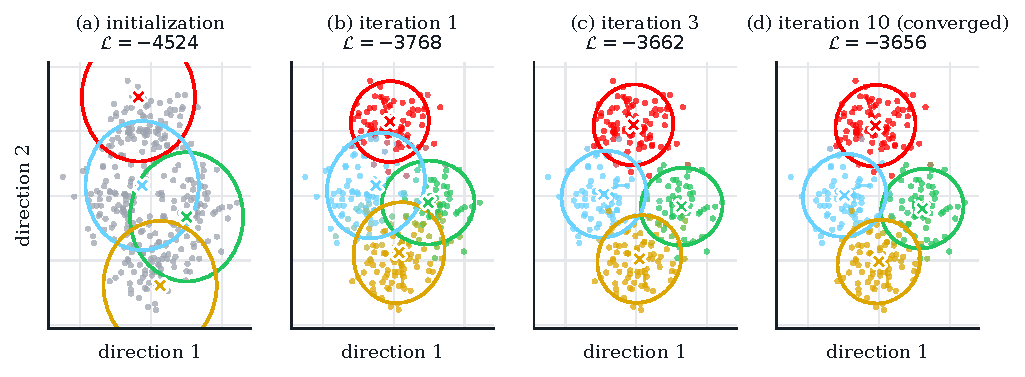
\includegraphics[width=0.9\textwidth]{../img/em-steps.pdf}

\small Diagonal model on \texttt{synth\_clean} ($D=10$, $K=4$), 2D projection. Colours = responsibilities, crosses = means with their path, ellipses = $2\sigma$ contours.

\medskip
An interactive step-by-step web page (\texttt{src/visual-sequential/}) runs the same EM and checks $\mathcal{L}$ of every iteration against the C binary.
\end{frame}

\begin{frame}{Diagonal vs full model}
\small
\resizebox{\textwidth}{!}{\begin{tabular}{lll}
\toprule
& \textbf{Diagonal} & \textbf{Full} \\
\midrule
Parameters per cluster & $\mu_k,\sigma_k^2$ \; ($2D$) & $\mu_k,\Sigma_k$ \; ($D+D(D+1)/2$) \\
Log-density & $-\tfrac12\sum_d[\ln 2\pi\sigma_{kd}^2+(x_d-\mu_{kd})^2/\sigma_{kd}^2]$ & $-\tfrac12[D\ln2\pi+\ln\det\Sigma_k+\|L_k^{-1}(x-\mu_k)\|^2]$ \\
Cost per iteration & $O(NKD)$ & $O(NKD^2)$ (+ $O(KD^3)$ Cholesky) \\
Bottleneck & memory & computation (large $D$) \\
\bottomrule
\end{tabular}}

\bigskip
\textbf{Full model: never invert $\Sigma_k$}
\begin{itemize}
\item Once per cluster and iteration: Cholesky $\Sigma_k=L_kL_k^\top$ ($D^3/6$).
\item Per point: forward substitution $L_k z=x_i-\mu_k$ ($D^2/2$), Mahalanobis $=\|z\|^2$, $\ln\det\Sigma_k=2\sum_d\ln L_{k,dd}$.
\item If a pivot is $\le 0$: jitter $\delta$ on the diagonal, $\times10$ until it succeeds (as \texttt{reg\_covar} in scikit-learn).
\end{itemize}
\end{frame}

% =====================================================================
\section{Parallel design}

\begin{frame}{Eight programs: four versions per model}
\small
\begin{tabular}{lp{0.70\textwidth}}
\toprule
\textbf{Version} & \textbf{What it is} \\
\midrule
\vseq{} & single process, single thread: correctness reference and serial time for speedup \\
\vbase{} & straightforward hybrid parallelization, two \texttt{MPI\_Allreduce} per iteration; reference for the optimizations \\
\optone{} (\textbf{computation}) & fused E+M step in one pass, one parallel region per iteration, no false sharing; \emph{full}: blocks of $B=64$ rows + SIMD forward substitution \\
\opttwo{} (\textbf{communication}) & ONE \texttt{MPI\_Allreduce} per iteration ($\mathcal{L}$ in the same buffer); \emph{full}: only the lower triangle of $\sum r xx^\top$ \\
\bottomrule
\end{tabular}

\bigskip
\begin{itemize}
\item Each optimization starts from \vbase{} of its own model and changes \textbf{one aspect only} $\Rightarrow$ its effect is isolated.
\item All versions of a model reach the \textbf{same iterations and the same $\mathcal{L}$} (relative difference $<10^{-8}$ over 14\,259 runs).
\end{itemize}
\end{frame}

\begin{frame}{Foster's methodology}
\begin{columns}[T]
\begin{column}{0.55\textwidth}
\footnotesize
\begin{description}
\item[Partitioning] task = one row of $X$ (E-step independent per row, M-step = sum over rows).
\item[Communication] only $\mathcal{L}$ and the M-step sums are global $\Rightarrow$ a \textbf{reduction} is enough.
\item[Agglomeration] $N$ rows in $P$ contiguous blocks, one per MPI rank; inside a rank one chunk per thread (\texttt{schedule(static)}: every row costs the same). Each rank \textbf{reads only its own block} from the file: no scatter.
\item[Mapping] parameters \textbf{replicated}; every rank recomputes them from the reduced sums $\Rightarrow$ \textbf{no broadcast}.
\end{description}
\end{column}
\begin{column}{0.43\textwidth}
\centering
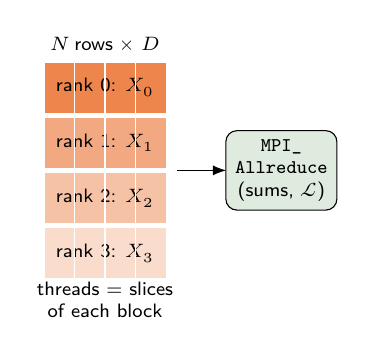
\begin{tikzpicture}[scale=0.7, every node/.style={font=\scriptsize}]
  \foreach \r/\c in {0/accent!70,1/accent!50,2/accent!35,3/accent!20} {
    \fill[\c] (0,-\r*1.0) rectangle (2.2,-\r*1.0-0.9);
    \node at (1.1,-\r*1.0-0.45) {rank \r: $X_\r$};
    \foreach \t in {0,1,2,3} \draw[white,thin] (2.2*\t/4,-\r*1.0) -- (2.2*\t/4,-\r*1.0-0.9);
  }
  \node[align=center] at (1.1,0.35) {$N$ rows $\times$ $D$};
  \draw[-{Latex}] (2.4,-1.95) -- (3.3,-1.95);
  \node[draw,rounded corners,fill=good!15,align=center] at (4.3,-1.95) {\texttt{MPI\_}\\\texttt{Allreduce}\\(sums, $\mathcal{L}$)};
  \node[align=center] at (1.1,-4.3) {threads = slices\\of each block};
\end{tikzpicture}
\end{column}
\end{columns}
\takeaway{Communication volume is $O(KD)$ or $O(KD^2)$ per iteration: it does \textbf{not} depend on $N$.}
\end{frame}

\begin{frame}{\vbase{}: what every rank does}
\footnotesize
\begin{enumerate}
\item Read own block $X_p$ ($\approx N/P$ rows). Initialization: every rank computes the same $K$ seeded indices, the owners copy the rows, one \texttt{Allreduce} (sum of zeros + rows) gives all $K$ rows to everyone.
\item For $t=1\ldots T_{\max}$:
  \begin{itemize}
  \item \textbf{E-step}: \texttt{omp parallel for reduction(+:$\ell$)} over local rows, stores $r_{ik}$ ($n_p\times K$).
  \item \texttt{MPI\_Allreduce}($\ell\to\mathcal{L}$, 1 double) $\to$ convergence test, \emph{same decision on all ranks}.
  \item \textbf{M-step}: \texttt{omp parallel for reduction(+:acc[0:len])}, acc $=[N_k\,|\,S\,|\,Q]$ (array reduction: private copy per thread).
  \item \texttt{MPI\_Allreduce}(acc): $K+2KD$ doubles (diag) or $K+KD+KD^2$ (full), packed in one buffer.
  \item Every rank updates $\pi,\mu,\Sigma$ by itself.
  \end{itemize}
\item \texttt{MPI\_Gatherv} of the labels on rank 0 (only for evaluation, not timed).
\end{enumerate}
MPI called only outside parallel regions: \texttt{MPI\_THREAD\_FUNNELED}.

\alert{Weak points}: two passes over the data, two synchronization points, per-thread buffers that can share a cache line (\texttt{malloc} aligns to 16 B) $\Rightarrow$ \textbf{false sharing}; full model: $K$ Cholesky by the master thread only.
\end{frame}

\begin{frame}{Optimization 1 --- computation}
\begin{columns}[T]
\begin{column}{0.5\textwidth}
\footnotesize
\textbf{Both models}
\begin{itemize}
\item \textbf{Fusion} of E- and M-step: responsibilities of a row used immediately, never stored. $X$ read \textbf{once} per iteration instead of twice.
\item \textbf{One parallel region} per iteration: cluster terms (and, full, the $K$ Cholesky) split among threads.
\item \textbf{No false sharing}: thread-local buffer (stack) / 64-byte aligned slices.
\item If converged, the sums of the last pass are discarded $\Rightarrow$ same iterations and $\mathcal{L}$.
\end{itemize}
\end{column}
\begin{column}{0.5\textwidth}
\footnotesize
\textbf{Full model only: blocks of $B=64$ rows}
\begin{itemize}
\item Row by row: forward substitution is a chain of dependent subtractions (no SIMD), $L_k$ re-read for each row, sums ($KD^2$) read/written per row.
\item Block transposed in a per-thread buffer ($D\times B$): forward substitution on \textbf{8 rows together} (8 independent chains in SIMD registers), each $L_{k,ab}$ loaded once for 8 rows.
\item Sums accumulated in registers over $B$ rows, \textbf{one write per block}.
\item BLAS level 2 (TRSV, SYR) $\to$ level 3 (TRSM, SYRK), by hand, inspired by Kwedlo 2023.
\item $B=64$: buffers $\approx(2D+2K)B$ doubles $\approx57$ KB, fit in L2 (1 MB).
\end{itemize}
\end{column}
\end{columns}
\end{frame}

\begin{frame}{Optimization 2 --- communication}
\footnotesize
\begin{itemize}
\item \textbf{One collective per iteration}: local $\ell$ written in an extra slot, $[N_k\,|\,S\,|\,Q\,|\,\ell]$, one \texttt{MPI\_Allreduce} (message aggregation).
\item M-step loop moved \emph{before} the convergence test; on the converged iteration the sums are discarded (one extra M-step loop per run). Computation identical to \vbase{} line by line.
\item \textbf{Full model}: only the lower triangle of every $Q_k$ is sent: $K D(D+1)/2$ instead of $KD^2$ (e.g.\ $K=6$, $D=50$: 120 KB $\to$ 61 KB).
\end{itemize}
\textbf{Why it should help --- cost model of Thakur et al.}
\begin{itemize}
\item Short message, recursive doubling: $\lg P\,(\alpha+n\beta+n\gamma)$. The removed call carries 1 double $\Rightarrow$ pure latency $\approx \lg P\,\alpha$ saved.
\item Long message, Rabenseifner: $2\lg P\,\alpha+2n\beta+n\gamma$ $\Rightarrow$ halving $n$ halves the bandwidth terms.
\item One synchronization point instead of two: fast ranks wait once per iteration.
\end{itemize}
\takeaway{Expected gain only where communication matters: several nodes, short iterations.}
\end{frame}

\begin{frame}{Data dependence analysis}
\footnotesize
For every OpenMP loop of the six parallel programs: \textbf{detection, classification, removal} (Chandra et al.).
\begin{columns}[T]
\begin{column}{0.5\textwidth}
\begin{itemize}
\item \textbf{Privatization} --- anti/output deps on scratch buffers (\texttt{logp}, $z$, \texttt{buf}, block buffers): one slice / local array per thread.
\item \textbf{Reduction} --- flow deps of $\mathcal{L}$ and acc: \texttt{reduction(+:ll)}, \texttt{reduction(+:acc[:len])}, \texttt{omp simd reduction}; between ranks \texttt{MPI\_Allreduce}.
\item \textbf{End of a loop} --- $r$ written by E-step loop, read by M-step loop: implicit barrier/join.
\end{itemize}
\end{column}
\begin{column}{0.5\textwidth}
\begin{itemize}
\item \textbf{Not removable} (recurrences):
  \begin{enumerate}
  \item EM loop over $t$: parallelism is \emph{inside} one iteration;
  \item forward substitution: $z_a$ needs $z_0..z_{a-1}$;
  \item Cholesky: element $(i,j)$ needs earlier ones.
  \end{enumerate}
  (2) and (3) are inside \emph{one} iteration of the parallel loop $\Rightarrow$ not loop-carried for it. \optone{} full still exploits parallelism around them: 8 rows per SIMD tile, $K$ factorizations split among threads.
\end{itemize}
\end{column}
\end{columns}
\takeaway{No unhandled dependence. Confirmed empirically: a race would give random, large differences, we see $<10^{-8}$.}
\end{frame}

% =====================================================================
\section{Experimental setup}

\begin{frame}{Hardware and measurement methodology}
\begin{columns}[T]
\begin{column}{0.47\textwidth}
\footnotesize
\textbf{HPC3 cluster} (PBS Pro, \texttt{shortCPUQ}), only \texttt{cpu\_type=Xeon6252N}
\begin{itemize}
\item 4 $\times$ Xeon Gold 6252N (Cascade Lake), 96 cores/node, 4 NUMA nodes, AVX-512
\item L1d 32 KB, L2 1 MB per core, L3 35.75 MB/socket
\item Ethernet 10 Gb/s between nodes
\item GCC 12.3 \texttt{-O3 -fopenmp}, Open MPI 4.1.5 + UCX over TCP
\item Binding: \texttt{--map-by slot:PE=$T$ --bind-to core}, \texttt{OMP\_PROC\_BIND=close}
\end{itemize}
\end{column}
\begin{column}{0.51\textwidth}
\footnotesize
\begin{itemize}
\item Metric: \textbf{time per iteration} $t_{\mathrm{it}}=(t_E+t_M+t_{\mathrm{comm}})/\text{iter}$ (max over ranks).
\item 3 repetitions, median, min--max bars; 3 warm-up iterations discarded.
\item \textbf{Exclusive nodes only}: \texttt{pack:excl} 1--8 cores, \texttt{scatter:excl} 16, 32 cores (2, 4 nodes).
\item \textbf{Fastest split} with $\ge 2$ ranks per node at every core count (1 rank/node failed: Open MPI binding on remote nodes).
\item Same seed (42), $K$, $\varepsilon$, $T_{\max}$ for every version.
\item Every run appends one log entry; all plots regenerated from the logs.
\end{itemize}
\end{column}
\end{columns}
\end{frame}

\begin{frame}{Datasets}
\footnotesize
\begin{columns}[T]
\begin{column}{0.5\textwidth}
\textbf{10 real datasets} (UCI, OpenML, BrainWeb), mostly medical: from 270 rows to 11.9 M voxels, $D$ from 1 to 20\,264. Z-score, numeric columns only.

\medskip
\alert{Problem}: 9 of 10 have $\le$ 254\,000 rows $\Rightarrow$ runs of 0.1 ms -- 0.1 s, mostly noise (median spread 8\% below 10 ms).

\medskip
Only \texttt{brainweb} (MRI, $N=11.9$ M, $D=1$, $K=12$) is large enough.
\end{column}
\begin{column}{0.5\textwidth}
\textbf{Synthetic} (known GMM, clinical-like variables, seed 42):

\smallskip
\begin{tabular}{lccc}
\toprule
& \texttt{clean} & \texttt{overlap} & \texttt{rare} \\
\midrule
$K$ / $D$ & 4 / 10 & 5 / 20 & 6 / 50 \\
Cov. & diag. & correlated & diag. \\
Tests & correct. & mismatch & rare cl., outliers \\
\bottomrule
\end{tabular}

\smallskip
Weak scaling: $N=250\,000\cdot p$, $p\in\{1,2,4,8,16\}$. Strong: \texttt{\_p08} (2 M) and \texttt{\_p16} (4 M) on 1--32 cores. Sweeps over $K$ and $D$.
\end{column}
\end{columns}
\takeaway{Rule: a dataset is shown only if \emph{every} run lasts $\geq 1$ s (spread of a few \%). All 14\,259 runs are kept in the logs.}
\end{frame}

\begin{frame}{Validation of the clustering}
\begin{columns}[c]
\begin{column}{0.55\textwidth}
\plot[1]{cluster/C2-choose-k.pdf}
\end{column}
\begin{column}{0.43\textwidth}
\small
\begin{itemize}
\item BIC/AIC minimum at the true $K=4$ on \texttt{synth\_clean}, both models.
\item ARI 0.91 on \texttt{synth\_clean}; on correlated \texttt{synth\_overlap} \textbf{full 0.85 vs diagonal 0.07}.
\item Real data: ARI $\le 0.14$ (labels are clinical outcomes, not Gaussian groups).
\item Iterations vary a lot (20 diag vs 56 full on \texttt{synth\_clean}, 200 on \texttt{brainweb}) $\Rightarrow$ metric = time \emph{per iteration}.
\end{itemize}
\end{column}
\end{columns}
\end{frame}

% =====================================================================
\section{Results}

\begin{frame}{Strong scaling --- diagonal model}
\perfplot{P4-strong-diagonal}
\begin{itemize}
\item The three parallel versions have almost the same time per iteration (32 cores: 0.107--0.115 s on \texttt{brainweb}, 17.3--17.6 ms on \texttt{synth\_overlap\_p08}).
\item Doubling the cores halves the time, also from 1 to 2 and 4 nodes.
\end{itemize}
\end{frame}

\begin{frame}{Strong scaling --- full model}
\perfplot{P4-strong-full}
\begin{itemize}
\item \optone{} $\approx$\textbf{2$\times$ faster} than \vbase{} at \emph{every} core count, already on 1 core (19.4 s vs 33.6 s of \vseq{} on \texttt{synth\_rare\_p16}).
\item \vbase{} and \opttwo{} share the computation $\Rightarrow$ same curve. On \texttt{brainweb} ($D=1$) nothing to block: \optone{} only 8--12\% faster.
\end{itemize}
\end{frame}

\begin{frame}{Speedup over \vseq{} --- diagonal model}
\perfplot{P2-speedup-diagonal}
\begin{itemize}
\item Ideal line up to 8 cores (6.8--7.7$\times$), keeps scaling across nodes: \textbf{27--29$\times$ on 32 cores}, efficiency 0.83--0.92, for all three versions.
\end{itemize}
\end{frame}

\begin{frame}{Speedup over \vseq{} --- full model}
\perfplot{P2-speedup-full}
\begin{itemize}
\item \vbase{}, \opttwo{}: \textbf{24--25.5$\times$} (eff.\ 0.75--0.80); on 1 core 0.85--0.88 (cost of the parallel structure, no gain).
\item \optone{}: \textbf{$\approx$50$\times$} (49.1--52.5, eff.\ 1.54--1.64). Not superlinear scaling: a $\approx$2$\times$ faster kernel $\times$ near-ideal scaling.
\end{itemize}
\end{frame}

\begin{frame}{Parallel efficiency}
\begin{columns}[c]
\begin{column}{0.5\textwidth}
\centering\small\textbf{Diagonal}\\
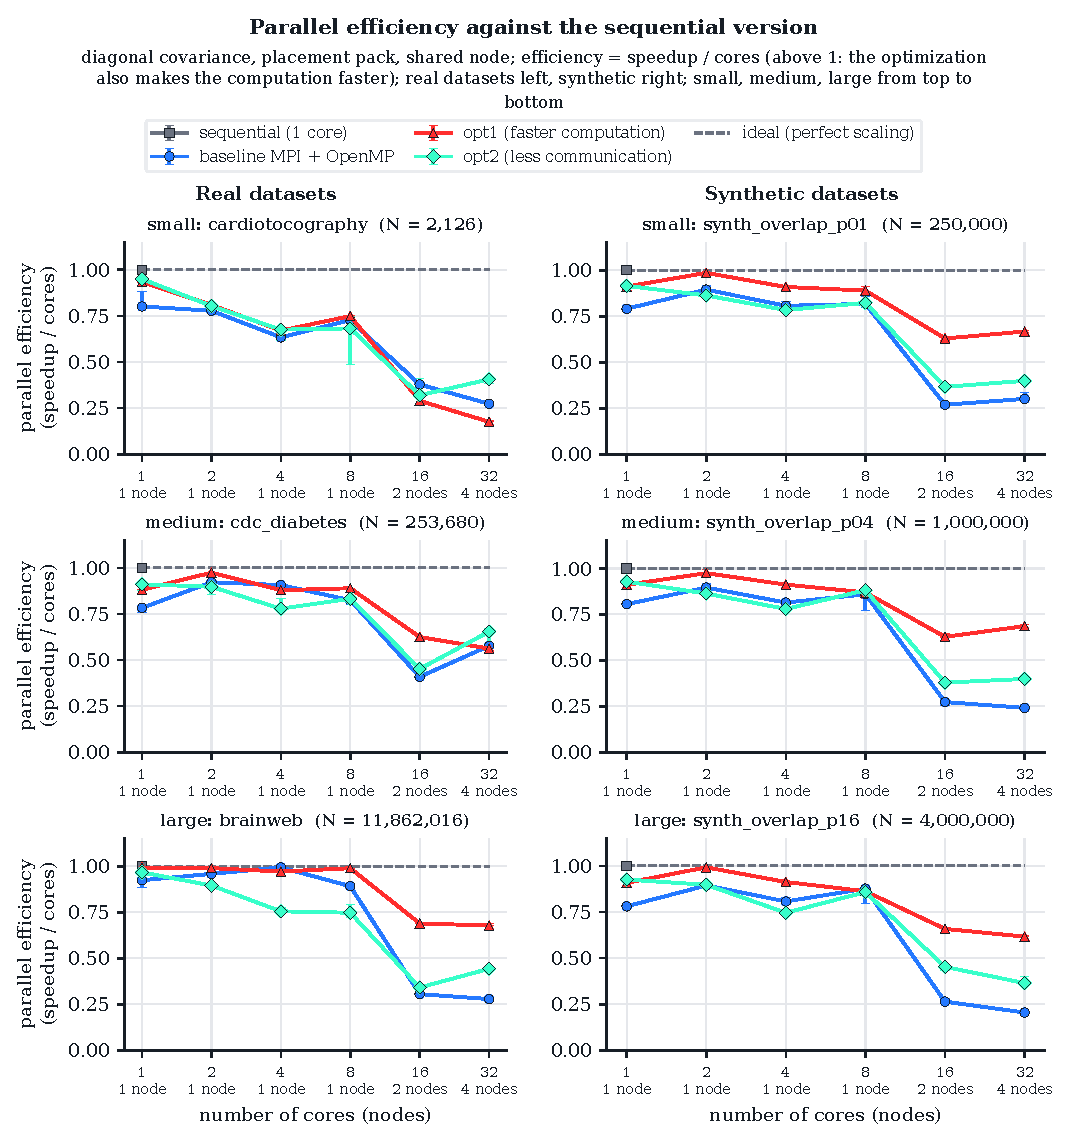
\includegraphics[width=\textwidth]{../../results/plots/performance/P3-efficiency-diagonal.pdf}
\end{column}
\begin{column}{0.5\textwidth}
\centering\small\textbf{Full}\\
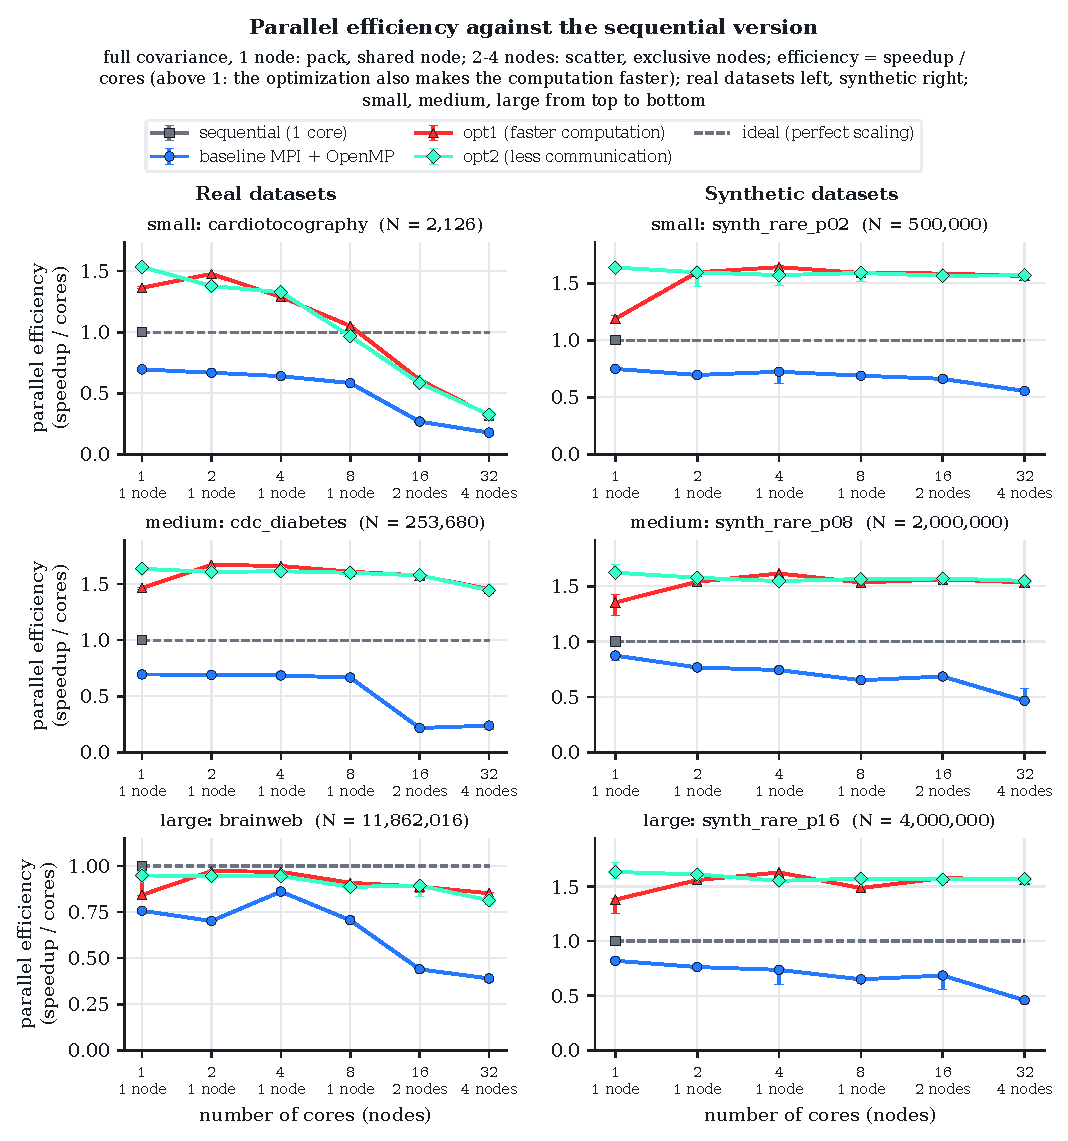
\includegraphics[width=\textwidth]{../../results/plots/performance/P3-efficiency-full.pdf}
\end{column}
\end{columns}
\begin{itemize}
\item Efficiency = speedup / cores, against \vseq{} of the same model and dataset.
\item No drop from 8 to 16 cores (1 $\to$ 2 nodes): up to 4 nodes the network does not slow down the scaling.
\end{itemize}
\end{frame}

\begin{frame}{Weak scaling}
\begin{columns}[c]
\begin{column}{0.34\textwidth}
\centering\small\textbf{Diagonal}\\
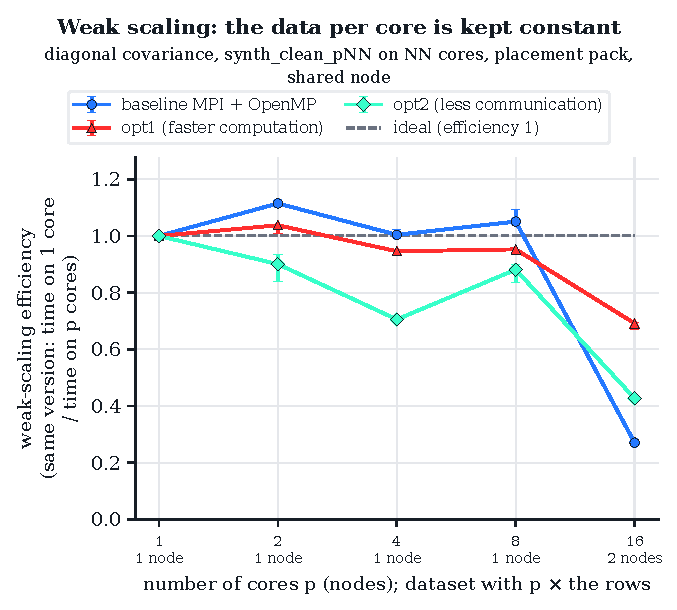
\includegraphics[width=\textwidth]{../../results/plots/performance/P5-weak-diagonal.pdf}
\end{column}
\begin{column}{0.34\textwidth}
\centering\small\textbf{Full}\\
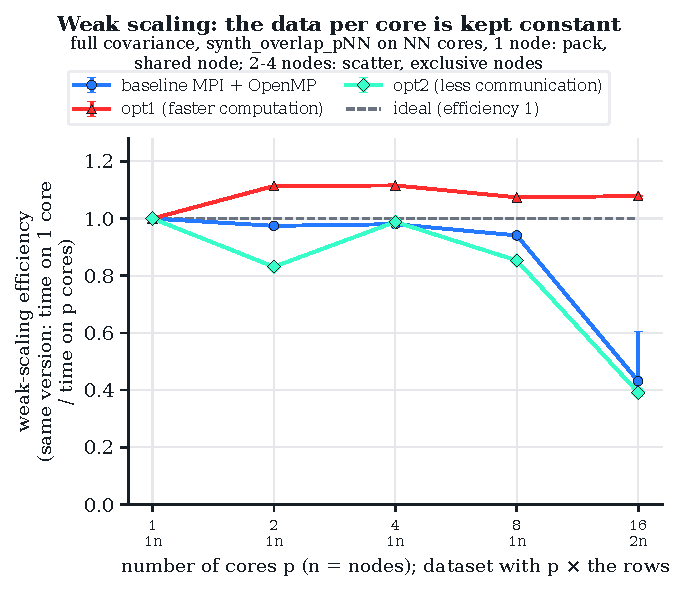
\includegraphics[width=\textwidth]{../../results/plots/performance/P5-weak-full.pdf}
\end{column}
\begin{column}{0.30\textwidth}
\small
\texttt{synth\_overlap\_p$NN$} on $NN$ cores: constant data per core ($250\,000$ rows). Efficiency = own time on 1 core / time on $p$ cores.
\begin{itemize}
\item diagonal: 0.87--0.99 on one node, 0.87--0.88 on 2 nodes;
\item full: 0.90--0.99, 0.90--0.92 on 2 nodes;
\item same for the three versions.
\end{itemize}
\end{column}
\end{columns}
\end{frame}

\begin{frame}{Gain of the optimizations --- diagonal model}
\perfplot{P9-opt-gain-diagonal}
\begin{itemize}
\item Time over \vbase{} on 32 cores: \optone{} 0.97--0.99 (0.92--1.00 on one node, at most 8\%), \opttwo{} 0.97--1.05 $\Rightarrow$ within job-to-job variation.
\end{itemize}
\end{frame}

\begin{frame}{Gain of the optimizations --- full model}
\perfplot{P9-opt-gain-full}
\begin{itemize}
\item \optone{}: \textcolor{good}{\textbf{0.48--0.51}} (1.95--2.07$\times$), same ratio on 1 and 8 cores: the gain is in every row, parallelization keeps it. In line with Kwedlo 2023 (1.75--2.75$\times$). 0.88 on \texttt{brainweb}.
\item \opttwo{}: 0.98--1.02.
\end{itemize}
\end{frame}

\begin{frame}{Roofline --- diagonal model (one node, 8 cores)}
\perfplot{P10-roofline-diagonal}
\begin{itemize}
\item Roofs: AVX-512 589, \emph{our SSE2 binaries} 74 GFLOP/s, STREAM 97 GB/s (analytic FLOP/bytes, lower bound).
\item All versions $\approx$23 GFLOP/s: the fusion of \optone{} raises the intensity 1.9 $\to$ 4.6 FLOP/B, not the speed.
\end{itemize}
\end{frame}

\begin{frame}{Roofline --- full model (one node, 8 cores)}
\perfplot{P10-roofline-full}
\begin{itemize}
\item \vbase{}/\opttwo{} 20--25 GFLOP/s, \optone{} 42--49 GFLOP/s: \textbf{2.0$\times$ more useful work per second} on the same node, 58--67\% of the SSE2 roof.
\end{itemize}
\end{frame}

\begin{frame}{Where the time goes --- diagonal model}
\perfplot{P8-breakdown-diagonal}
\begin{itemize}
\item $t_{\mathrm{comm}}$ $\le$ 9\% on one node, $\le$ 11\% on 32 cores --- and it \emph{includes the wait} for the slowest rank.
\item Reading the dataset: $\le$ 2\% on one node, up to 6\% on 32 cores.
\end{itemize}
\end{frame}

\begin{frame}{Where the time goes --- full model}
\perfplot{P8-breakdown-full}
\begin{itemize}
\item \vbase{} on \texttt{synth\_rare}: M-step is 40--41\% (the $\Sigma_k$ sums cost as much as the distances). \optone{}: one fused pass, almost all ``E-step''.
\end{itemize}
\end{frame}

\begin{frame}{Communication: wait vs collectives}
\small
Per-rank compute times are logged $\Rightarrow$ $t_{\mathrm{comm}}$ split into \textbf{wait} (slowest $-$ fastest rank) and real cost of the \textbf{collectives}. Per iteration, 32 cores (4 nodes, \texttt{scatter:excl}), medians over the long datasets:

\medskip
\centering
\begin{tabular}{llccc}
\toprule
Split per node & Model & \vbase{} & \optone{} & \opttwo{} \\
\midrule
2 ranks $\times$ 4 threads & diagonal & 0.60 ms & 0.33 ms & \textcolor{good}{\textbf{0.08 ms}} \\
                          & full     & 6.5 ms  & 0.58 ms & \textcolor{good}{\textbf{0.50 ms}} \\
8 ranks $\times$ 1 thread & diagonal & 0.62 ms & 0.38 ms & 0.38 ms \\
                          & full     & 1.57 ms & 0.62 ms & 0.77 ms \\
\bottomrule
\end{tabular}

\raggedright
\begin{itemize}
\item \opttwo{} does what it was designed for, \textbf{but} the collectives are \textbf{at most 4\%} of an iteration.
\item \optone{} full sends the same two messages as \vbase{} yet costs almost as little as \opttwo{}: most of the cost of \vbase{} is the \emph{second synchronization point}, not the bytes.
\end{itemize}
\end{frame}

\begin{frame}{Rank/thread split and load imbalance}
\begin{columns}[c]
\begin{column}{0.55\textwidth}
\centering\small\textbf{Imbalance between ranks, \opttwo{} diagonal}\\
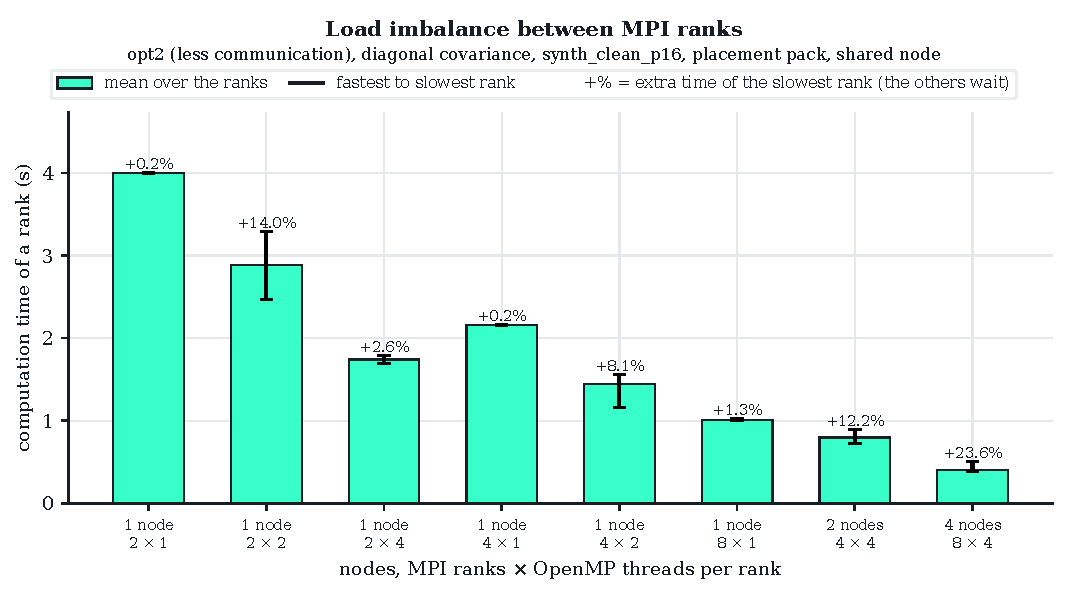
\includegraphics[width=\textwidth]{../../results/plots/performance/P11-imbalance-diagonal.pdf}
\end{column}
\begin{column}{0.44\textwidth}
\small
\begin{itemize}
\item \vbase{}, \opttwo{}: fastest with \textbf{1 thread per rank}; with 2 r $\times$ 4 t up to \textbf{1.9$\times$ slower} on one node, ranks imbalanced (6--19\% median), others wait 8--111 ms/iteration.
\item Cause: \textbf{false sharing} of per-thread buffers + (full) Cholesky on the master thread only.
\item \optone{} removed both: \textbf{within 7\%} across splits, balanced within 2.5\%.
\item Not the hardware: ranks on 4- and 6-channel nodes within 1\% of each other.
\end{itemize}
\end{column}
\end{columns}
\end{frame}

% =====================================================================
\section{Discussion and conclusion}

\begin{frame}{Discussion}
\small
\begin{description}
\item[Size decides] On the real medical tables \vseq{} is enough (runs of milliseconds). The parallel versions pay off from $\approx$0.5 M rows (full) and $\approx$2 M rows (diagonal).
\item[Computation is the bottleneck] \optone{} full is 2$\times$ faster at every core count because every core does more useful work. In the diagonal model there is nothing to block.
\item[Communication is not] \opttwo{} works as designed and removes most of the collective cost, but collectives are $\le$4\% of an iteration on these datasets and this network. Its regime (short iterations on many nodes) is exactly the noisy one we excluded.
\item[Threads need care] False sharing, not the memory of the nodes, explains the slow and imbalanced thread-heavy splits.
\end{description}
\textbf{Related work}: \vbase{} with 8 threads has efficiency 0.39--0.53, like Sanderson \& Curtin ($\approx$0.63 on 16 threads); \optone{} without false sharing 0.91--0.94. Kwedlo's blocked variant 1.75--2.75$\times$ vs our 2.0--2.1$\times$.
\end{frame}

\begin{frame}{Conclusion and future work}
\begin{columns}[T]
\begin{column}{0.52\textwidth}
\small
\textbf{Results}
\begin{itemize}
\item Hybrid MPI + OpenMP EM, 2 models $\times$ 4 versions, \textbf{correct} in all 14\,259 runs ($\Delta\mathcal{L}<10^{-8}$).
\item Speedup on 32 cores: \textbf{27--29$\times$} diagonal, \textbf{24--25$\times$} full, \textbf{$\approx$50$\times$} full with \optone{}.
\item Weak scaling efficiency $\ge$ 0.87 up to 16 cores.
\item Optimizing the computation pays; optimizing communication is correct but marginal here.
\end{itemize}
\end{column}
\begin{column}{0.46\textwidth}
\small
\textbf{Future work}
\begin{itemize}
\item Combine \optone{} and \opttwo{}.
\item Automatic choice of model/version/layout from the dataset (size, correlations, memory, BIC on a sample).
\item Lift the memory limit of the full model for large $D$ (shared sums, covariances split among ranks).
\item Rows distributed by measured rank speed.
\item Blocked full model on GPUs; more nodes, larger real data.
\end{itemize}
\end{column}
\end{columns}
\end{frame}

\begin{frame}[standout]
Thank you!\\[1em]
\normalsize Questions?
\end{frame}

% =====================================================================
\appendix
\backuptrue
\section{Backup slides}

\begin{frame}[fragile]{Backup: \vbase{} diagonal, pseudocode (rank $p$)}
\scriptsize
\begin{verbatim}
read X_p (n_p ~ N/P contiguous rows)            // no scatter
init: same K seeded indices on all ranks; owners copy rows; Allreduce(SUM)
for t = 1 .. T_max:
    c_k, iv_kd  (master thread)
    #pragma omp parallel for schedule(static) reduction(+:l)
    for i in X_p:  v_k = c_k - 1/2 sum_d (x_id - mu_kd)^2 iv_kd
                   m = log_sum_exp(v);  l += m;  r_ik = exp(v_k - m)
    MPI_Allreduce(l -> L, 1, SUM)                       // comm 1
    if |L - L_prev| <= eps |L|: break                   // all ranks together
    #pragma omp parallel for schedule(static) reduction(+:acc[0:K+2KD])
    for i in X_p:  acc = [N_k | S | Q] += [r_ik | r_ik x_id | r_ik x_id^2]
    MPI_Allreduce(IN_PLACE, acc, K+2KD, SUM)            // comm 2
    update pi, mu, sigma^2 on every rank (no broadcast); L_prev = L
MPI_Gatherv(labels -> rank 0)                           // not timed
\end{verbatim}
\normalsize
\opttwo{}: M-step loop before the test, $\ell$ in \texttt{acc[K+2KD]}, one \texttt{Allreduce} of $K+2KD+1$ doubles.\\
\optone{}: one \texttt{omp parallel} region, one fused loop, \texttt{double buf[K]} on the thread stack.
\end{frame}

\begin{frame}{Backup: why false sharing in \vbase{}?}
\small
\begin{itemize}
\item Per-thread buffers of the $K$ log-densities are \emph{slices of one allocated array}.
\item Each slice is padded to a multiple of 64 bytes, but \texttt{malloc} aligns the array only to \textbf{16 bytes} $\Rightarrow$ slices are not aligned to cache lines.
\item Two neighbouring slices can share one 64-byte line at their boundary: every write of a thread invalidates the line in the other core's cache (coherence traffic, MESI).
\item Effect grows with the number of threads per rank $\Rightarrow$ 1 thread per rank is fastest, thread-heavy splits are slow and imbalanced.
\item \optone{} diagonal: buffer is a local array of each thread (own stack). \optone{} full: buffers allocated once, \textbf{64-byte aligned}, every slice a multiple of 64 B.
\end{itemize}
\takeaway{Evidence: OpenMP-only (1 rank $\times$ 8 threads) \vbase{} diagonal reaches 3.1--4.2$\times$, \optone{} 7.3--7.5$\times$.}
\end{frame}

\begin{frame}{Backup: correctness and reproducibility}
\small
\begin{itemize}
\item All versions, layouts, placements: 7\,275 runs (diagonal) + 6\,984 (full).
\item Number of iterations \textbf{identical} on every dataset.
\item Max relative difference of $\mathcal{L}$ vs \vseq{}: $5.1\cdot10^{-9}$ (diag), $7.7\cdot10^{-9}$ (full), both on \texttt{brainweb} (200 iterations). Elsewhere $\le 1.5\cdot10^{-10}$ (full), 0 to the logged digits (diag).
\item Differences only from the \textbf{order of floating-point sums} (threads, ranks, blocks).
\item \optone{} full: per-row Mahalanobis operations in the same order as \vbase{} $\Rightarrow$ bitwise identical; only the sums are reordered ($\sim10^{-12}$).
\item \opttwo{} full: with 1 rank bitwise identical; with more, MPI may pick another reduction algorithm for the different message size.
\item Same initial rows on every rank thanks to the seeded generator: no communication needed to agree.
\end{itemize}
\end{frame}

\begin{frame}{Backup: why the stability rule ($\geq 1$ s)}
\small
Spread of 3 repetitions, (max$-$min)/median, all layouts:
\begin{center}
\begin{tabular}{lc}
\toprule
Run duration & Median spread \\
\midrule
$<$ 10 ms & 8.2\% (above 70\% in 1 layout out of 10) \\
10--100 ms & 4.0\% \\
$>$ 1 s & 1.7\% (1.0\% one exclusive node, 2.4\% reserved multi-node) \\
\bottomrule
\end{tabular}
\end{center}
\begin{itemize}
\item Short runs measure fixed costs (thread start, MPI latency) and machine noise: differences between versions are of the same order as the noise.
\item Placement matters too: \texttt{scatter} on shared nodes has 22\% median spread; on one shared node \vbase{}/\opttwo{} full are 15--22\% slower than on an exclusive one $\Rightarrow$ only exclusive placements in the figures.
\item Nothing deleted: \texttt{--min-run 0} redraws every figure with all datasets.
\end{itemize}
\end{frame}

\begin{frame}{Backup: cost sweeps and dataset size}
\begin{columns}[c]
\begin{column}{0.5\textwidth}
\centering\small\textbf{P1 sweep, full model}\\
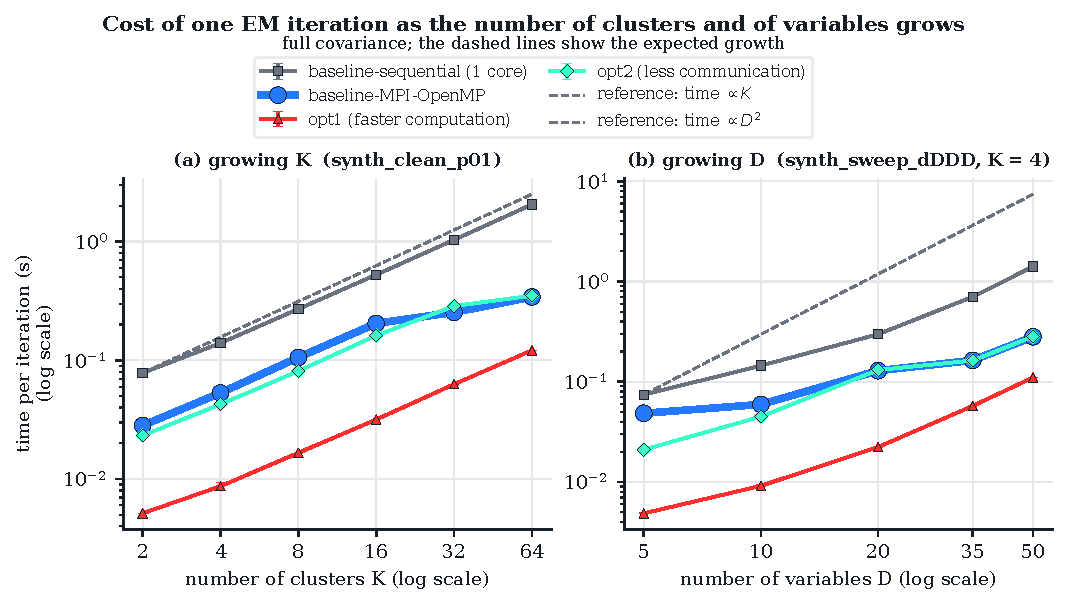
\includegraphics[width=\textwidth]{../../results/plots/performance/P1-sweep-full.pdf}
\end{column}
\begin{column}{0.5\textwidth}
\centering\small\textbf{P12 speedup vs rows, diagonal}\\
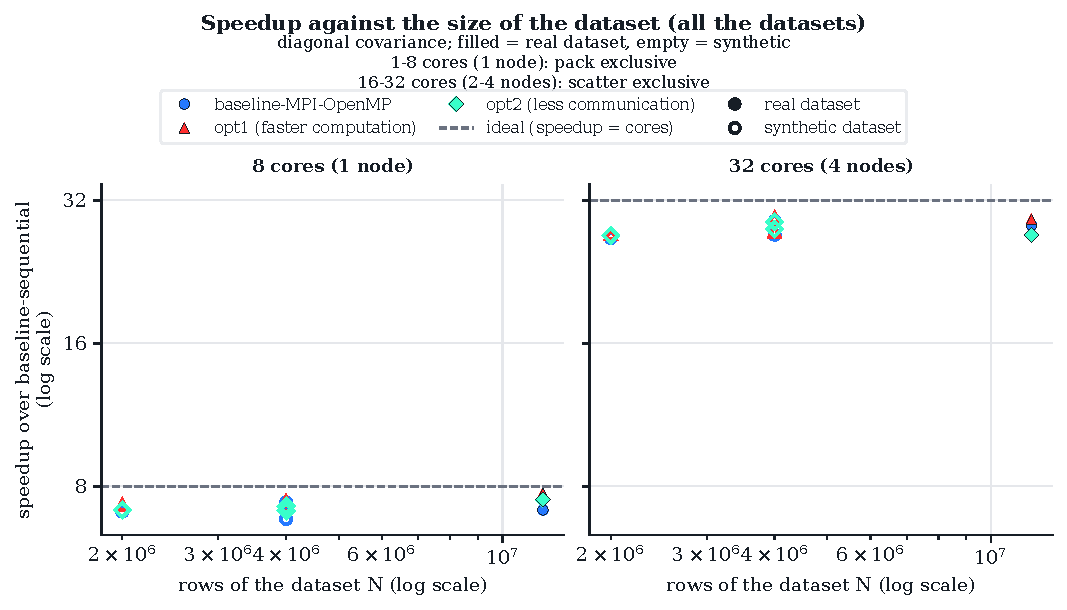
\includegraphics[width=\textwidth]{../../results/plots/performance/P12-size-diagonal.pdf}
\end{column}
\end{columns}
\small
\begin{itemize}
\item Time grows linearly in $K$, as $D$ (diagonal) or $D^2$ (full): confirms $O(NKD)$ / $O(NKD^2)$.
\item Smallest tables: 32 cores slower than one (diagonal); up to $\sim10^5$ rows speedup $\le 20$ on 32 cores.
\end{itemize}
\end{frame}

\begin{frame}{Backup: placement and ranks $\times$ threads (one node)}
\begin{columns}[c]
\begin{column}{0.4\textwidth}
\centering\small\textbf{P6 placement, full}\\
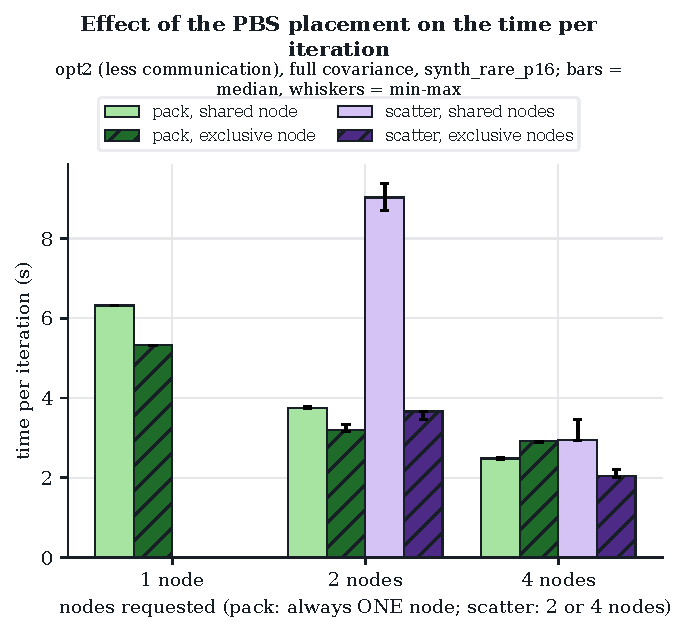
\includegraphics[width=0.95\textwidth]{../../results/plots/performance/P6-placement-full.pdf}
\end{column}
\begin{column}{0.4\textwidth}
\centering\small\textbf{P7 ranks $\times$ threads, full}\\
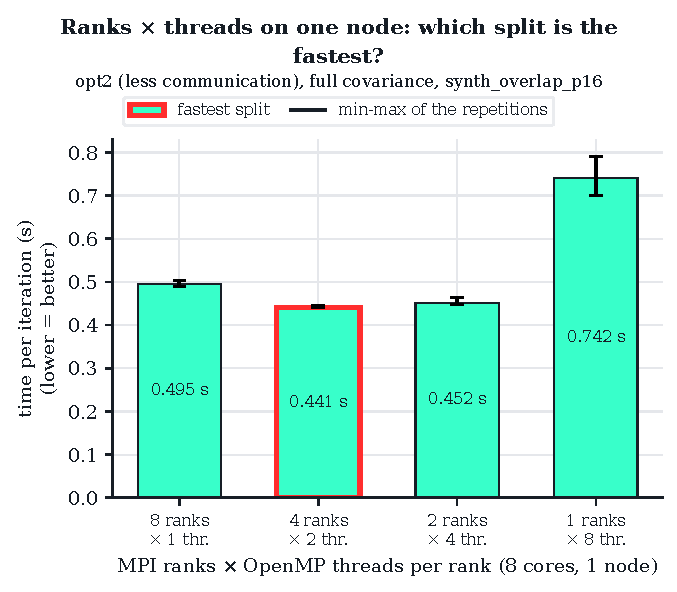
\includegraphics[width=0.95\textwidth]{../../results/plots/performance/P7-ranks-threads-full.pdf}
\end{column}
\end{columns}
\small
\begin{itemize}
\item \texttt{pack} puts the 2/4 chunks on \emph{one} node (96 cores): only \texttt{scatter} spreads over nodes.
\item Without \texttt{:excl}, ranks on remote nodes are not confined to reserved cores $\Rightarrow$ unreliable times.
\end{itemize}
\end{frame}

\begin{frame}{Backup: why no \texttt{gene\_rnaseq} with the full model}
\small
\begin{itemize}
\item $D=20\,264$: one $\Sigma_k$ has $D^2\approx4\cdot10^8$ values $\approx$ 3.3 GB; with $K=5$ $\approx$ 16 GB.
\item Three such arrays ($\Sigma_k$, $L_k$, sums) $\approx$ 50 GB \textbf{per MPI process}, plus a private copy of the sums ($\approx$16 GB) \textbf{per thread} for the array reduction $\Rightarrow$ 180--520 GB per node.
\item Statistically meaningless anyway: $N=801\ll D$, each $\Sigma_k$ has rank $\le N_k-1<D$, invertible only thanks to $\delta$; $\approx10^9$ parameters from 801 points.
\item Diagonal model is fine: second message $\approx$ 1.6 MB (bandwidth-bound, \opttwo{} saves relatively little).
\end{itemize}
\end{frame}

\begin{frame}{Backup: limits of the measurements}
\small
\begin{itemize}
\item One PBS job per (version, layout): nodes chosen by PBS. Two versions with the same computation (\vbase{} vs \opttwo{}) differ by $\le$ 2.6\% on one core $\Rightarrow$ job-to-job variability.
\item CPU frequency (turbo) not fixed; network shared with other users.
\item Memory configuration of the nodes not chosen (2/4/6 channels): checked afterwards, no effect, but only with 8 of the 24 cores of a socket.
\item 1-rank-per-node layouts failed on multi-node (Open MPI binding) $\Rightarrow$ excluded everywhere; on one node this changes the best split by $\le$ 8\%.
\item Stop at 4 nodes. Binaries compiled without \texttt{-march} (SSE2): AVX-512 left on the table.
\item Roofline FLOP/bytes are an analytic lower bound.
\end{itemize}
\end{frame}

\begin{frame}{AI statement and references}
\scriptsize
\textbf{AI statement.} We used an AI assistant (Claude, by Anthropic) for: (i) support in writing and debugging the code; (ii) searching sources and papers for the state of the art and the datasets; (iii) mathematical and grammatical correction of the report. Design choices, experiments and analysis are our own, and we reviewed the output of the assistant.

\medskip
\textbf{Main references}
\begin{itemize}
\item C. M. Bishop, \emph{Pattern Recognition and Machine Learning}, Springer, 2006, ch.~9.
\item C. Sanderson, R. Curtin, multi-threaded GMM/EM in C++, ICSPCS 2017.
\item W. Kwedlo, EM for GMM with linear algebra libraries on shared-memory systems, FedCSIS 2023.
\item S. X. Lee et al., multithreaded EM (2016) and multi-node EM (2020), arXiv.
\item L. Machlica et al., GMM estimation on GPU with CUDA, PDCAT 2011.
\item R. Thakur, R. Rabenseifner, W. Gropp, Optimization of collective communication in MPICH, IJHPCA 2005.
\item R. Chandra et al., \emph{Parallel Programming in OpenMP}, Morgan Kaufmann, 2001.
\end{itemize}
Full list, report and code: \url{https://github.com/HPC-2627/ParallelExpectationMaximizationClustering}
\end{frame}

\end{document}
